\section{Resultados Obtenidos}
\label{chap:resultados}

En esta sección se brinda un resumen de los resultados obtenidos al realizar los experimentos y se presentan ejemplos visuales de los experimentos.

\subsection{Resultados numéricos}

A continuación se muestran los resultados promedios obtenidos para los $VP$, $FP$, $VN$ y $FN$ en la Tabla \ref{resultados} (Ver resultados de manera extensiva en el Anexo \ref{chap:ApendiceA}). Los valores presentados muestran que el ordenamiento \textbf{MEDIANA-CIELAB} obtuvo los mayores resultados para las cuatro variables a considerar. En todos los resultados para los distintos métodos existe una gran cantidad de $FP$, esto indica que al realizar la segmentación los objetos obtenidos son de un tamaño mayor a los objetos en la imagen ideal. En los resultados se observa también que los métodos \textbf{MEDIANA-CIELAB} y \textbf{MEDIA-CIELAB} fueron los únicos que obtuvieron una cantidad mayor al 40\% en $VP$ por lo cual la distancia a colores de referencia que utilizan información de la imagen, como la mediana y la media, son los más adecuados para la segmentación de los amastigotes de Trypanosoma Cruzi.

\begin{table*}[]
\centering
\caption{Resultados de la Comparación}
\label{resultados}
\resizebox{15cm}{!} {
\begin{tabular}{|l|l|l|l|l|}
\hline
\multicolumn{1}{|c|}{\textbf{Método}} & \multicolumn{1}{c|}{\textbf{FP}} & \multicolumn{1}{c|}{\textbf{VP}} & \multicolumn{1}{c|}{\textbf{FN}}	&	\multicolumn{1}{c|}{\textbf{VN}} \\ \hline
\textbf{MEDIANA-CIELAB} & 53.9871 & 46.0129 & 3.241 & 96.759\\ \hline
\textbf{MEDIA-CIELAB} & 58.0464 & 41.9536 & 3.8889 & 96.1111\\ \hline
\textbf{DISTANCIA-EUCLIDIANA-CIELAB} & 62.382 & 37.618 & 3.388 & 96.612\\ \hline
\textbf{LEXICOGRAFICO-RGB} & 62.5968 & 37.4032 & 4.5841 & 95.4159\\ \hline
\textbf{ALGORITMO-MEYER} & 61.9621 & 38.0379 & 4.2933 & 95.7067 \\ \hline
\textbf{ALPHA-MOD-LEXICOGRAFICO-RGB} & 64.4714 & 32.6382 & 4.7328 & 95.2672\\ \hline
\textbf{DISTANCIA-EUCLIDIANA-RGB} & 64.4714 & 35.5286 & 4.6877 & 95.3123 \\ \hline
\textbf{ESCALA-DE-GRISES} & 62.4645 & 37.5355 & 4.9666 & 95.0334 \\ \hline
\textbf{VAZQUEZ-ET-AL} & 66.7119 & 33.2881 & 4.8933 & 95.1067\\ \hline
\textbf{ENTRELAZADO-RGB} & 67.171 & 32.829 & 5.5399 & 94.4601 \\ \hline
\textbf{LEXICOGRAFICO-HSI} & 65.1106 & 34.8894 & 5.6917 & 94.3083 \\ \hline
\textbf{ENTROPIA-RGB} & 66.6292 & 33.3708 & 5.5686 & 94.4314 \\ \hline
\textbf{MAXIMO-RGB} & 67.0666 & 32.9334 & 5.0553 & 94.9447 \\ \hline
\textbf{MINIMO-RGB} & 65.8297 & 34.1703 & 5.6771 & 94.3229 \\ \hline
\textbf{MODA-RGB} & 64.8527 & 35.1473 & 4.6959 & 95.3041 \\ \hline
\textbf{MODA-MAXIMO-RGB} & 64.8527 & 35.1473 & 4.6959 & 95.3041 \\ \hline
\textbf{MODA-MINIMO-RGB} & 64.8527 & 35.1473 & 4.6959 & 95.3041 \\ \hline
\textbf{SUAVIDAD-RGB} & 67.6638 & 32.3362 & 4.4133 & 95.5867 \\ \hline
\textbf{VARIANZA-RGB} & 66.7964 & 33.2036 & 4.8919 & 95.1081 \\ \hline
\end{tabular}
}
\end{table*}

La comparación de las métricas de sensibilidad, exactitud y especificidad de la implementación utilizando distintos métodos de orden entre píxeles, se puede observar en la Tabla \ref{resultadosCielab}. Los valores indican el promedio obtenido por cada método de ordenamiento para todas las imágenes.El método \textbf{MEDIANA-CIELAB} presenta una mejora de 3.14\% en Especificidad y 1.34\% en Exactitud en comparación con el siguiente mejor método. 


\begin{table}[!htb]
\centering
\caption{Resultados en espacio de color CIELab}
\label{resultadosCielab}
\resizebox{15cm}{!} {
\begin{tabular}{|l|l|l|l|}
\hline
\multicolumn{1}{|c|}{\textbf{Método}} & \multicolumn{1}{c|}{\textbf{$SEN$}}& \multicolumn{1}{c|}{\textbf{$ESP$}}&  \multicolumn{1}{c|}{\textbf{$EX$}}  \\ \hline
\textbf{MEDIANA-CIELAB} & 26.18\%  & 93.19\%  & 91.14\%  \\ \hline
\textbf{MEDIA-CIELAB} & 27.14\%  & 92.95\% & 90.94\%  \\ \hline
\textbf{DISTANCIA-EUCLIDIANA-CIELAB} & 27.24\%  & 91.76\% & 89.80\% \\ \hline
\textbf{LEXICOGRAFICO-RGB} & 27.41\%  & 90.05\% & 88.17\% \\ \hline
\textbf{ALGORITMO-MEYER} & 27.02\%  & 90.40\%  & 88.48\% \\ \hline
\textbf{ALPHA-MOD-LEXICOGRAFICO-RGB} & 27.31\% & 89.14\% & 87.27\% \\ \hline
\textbf{DISTANCIA-EUCLIDIANA-RGB} & 27.40\% & 88.73\% & 86.8\%  \\ \hline
\textbf{ESCALA-DE-GRISES} & 25.5\%  & 88.69\%  & 86.81\%  \\ \hline
\textbf{VAZQUEZ-ET-AL} & 27.37\%  & 88.08\%  & 86.25\% \\ \hline
\textbf{ENTRELAZADO-RGB} & 27.27\% & 88.02\% & 86.17\% \\ \hline
\textbf{LEXICOGRAFICO-HSI} & 27.39\%  & 87.96\% & 86.15\%  \\ \hline
\textbf{ENTROPIA-RGB} & 27.24\%  & 87.53\%  & 85.73\% \\ \hline
\textbf{MAXIMO-RGB} & 27.36\%  & 87.40\%  & 85.62\%  \\ \hline
\textbf{MINIMO-RGB} & 27.53\%  & 87.95\%  & 86.15\%  \\ \hline
\textbf{MODA-RGB} & 27.48\%  & 89.03\%  & 87.15\% \\ \hline
\textbf{MODA-MAXIMO-RGB} & 27.48\%  & 89.03\% & 87.15\%   \\ \hline
\textbf{MODA-MINIMO-RGB} & 27.48\%  & 89.03\% &  87.15\%   \\ \hline
\textbf{SUAVIDAD-RGB} & 27.55\% & 88.17\%  & 86.34\% \\ \hline
\textbf{VARIANZA-RGB} & 27.47\%  & 88.17\%  & 86.34\% \\ \hline
\end{tabular}
}
\end{table}

Para obtener un detalle de los datos se contabilizó además la cantidad total de imágenes en las que cada espacio (3 métodos en CIELab, 14 métodos en RGB y 1 método en HSI) de color obtuvo el mejor exactitud (ver Figura \ref{exp:exactitud}). En este conteo se puede ver que el espacio de color CIELab obtuvo la mejor segmentación en la mayor cantidad de las imágenes.

\begin{figure}[h!]
\centering
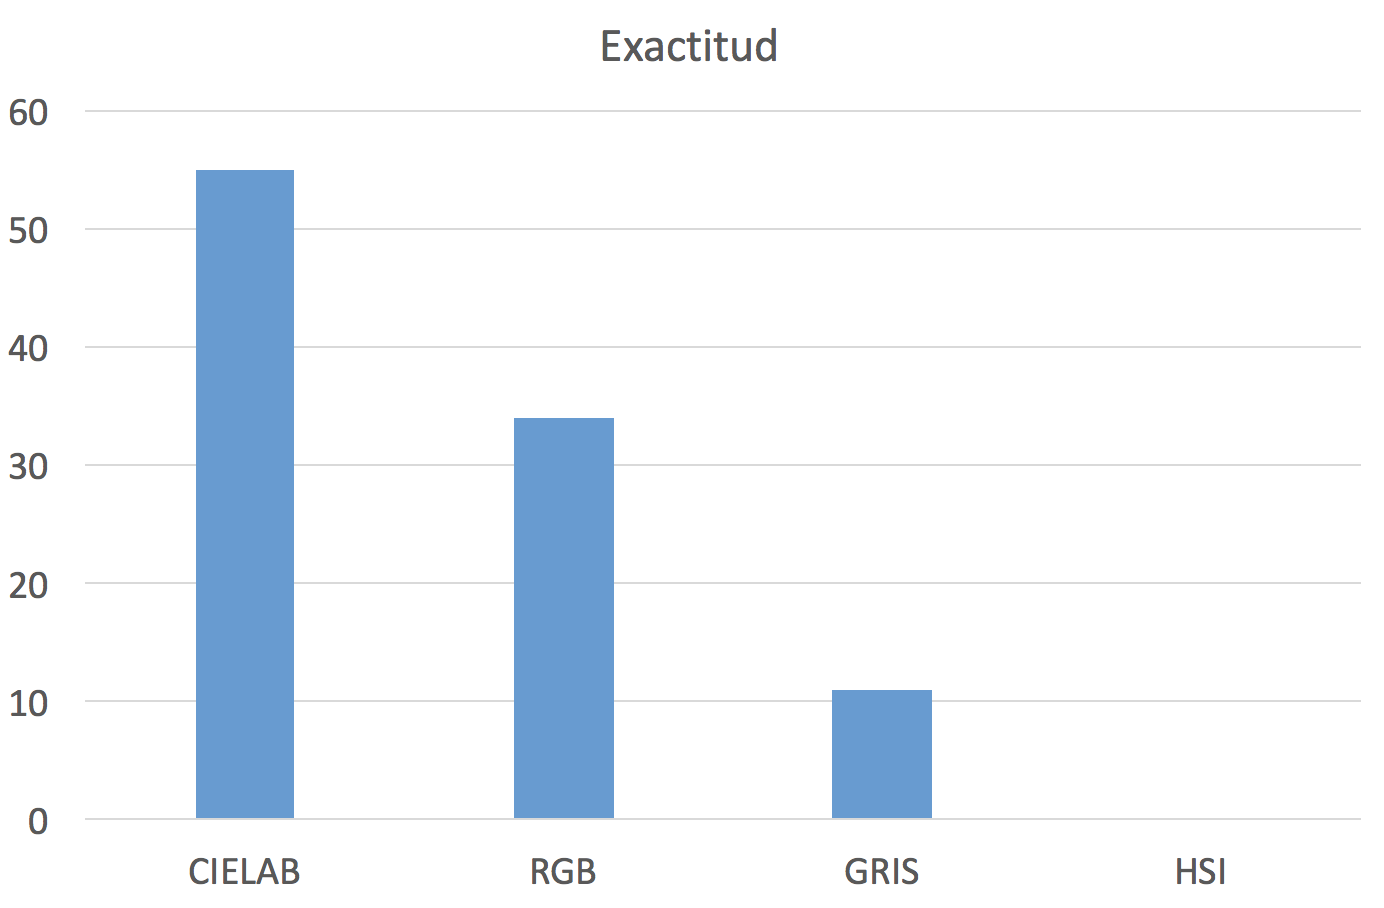
\includegraphics[width=160mm]{./imagenes/exactitud.png}
\caption{Cantidad de imágenes que dan el mejor resultado en exactitud por método}
\label{exp:exactitud}
\end{figure}

\subsection{Resultados visuales}

A continuación se muestran los ejemplos visuales de los experimentos realizados en el trabajo. La Figura \ref{exp:lab} muestra los resultados obtenidos en el espacio de color CIELab. En la Figura \ref{exp:lab}(a) se muestra una imagen del caso de estudio. Además se muestra la gradiente en la Figura \ref{exp:lab}(b) utilizada para la segmentación. La segmentación obtenida en la Figura \ref{exp:lab}(c) y la segmentación ideal se muestran en la Figura \ref{exp:lab} (d). Este ejemplo será utilizado posteriormente para la comparación con los distintos experimentos realizados.

\begin{figure}[h!]
\centering
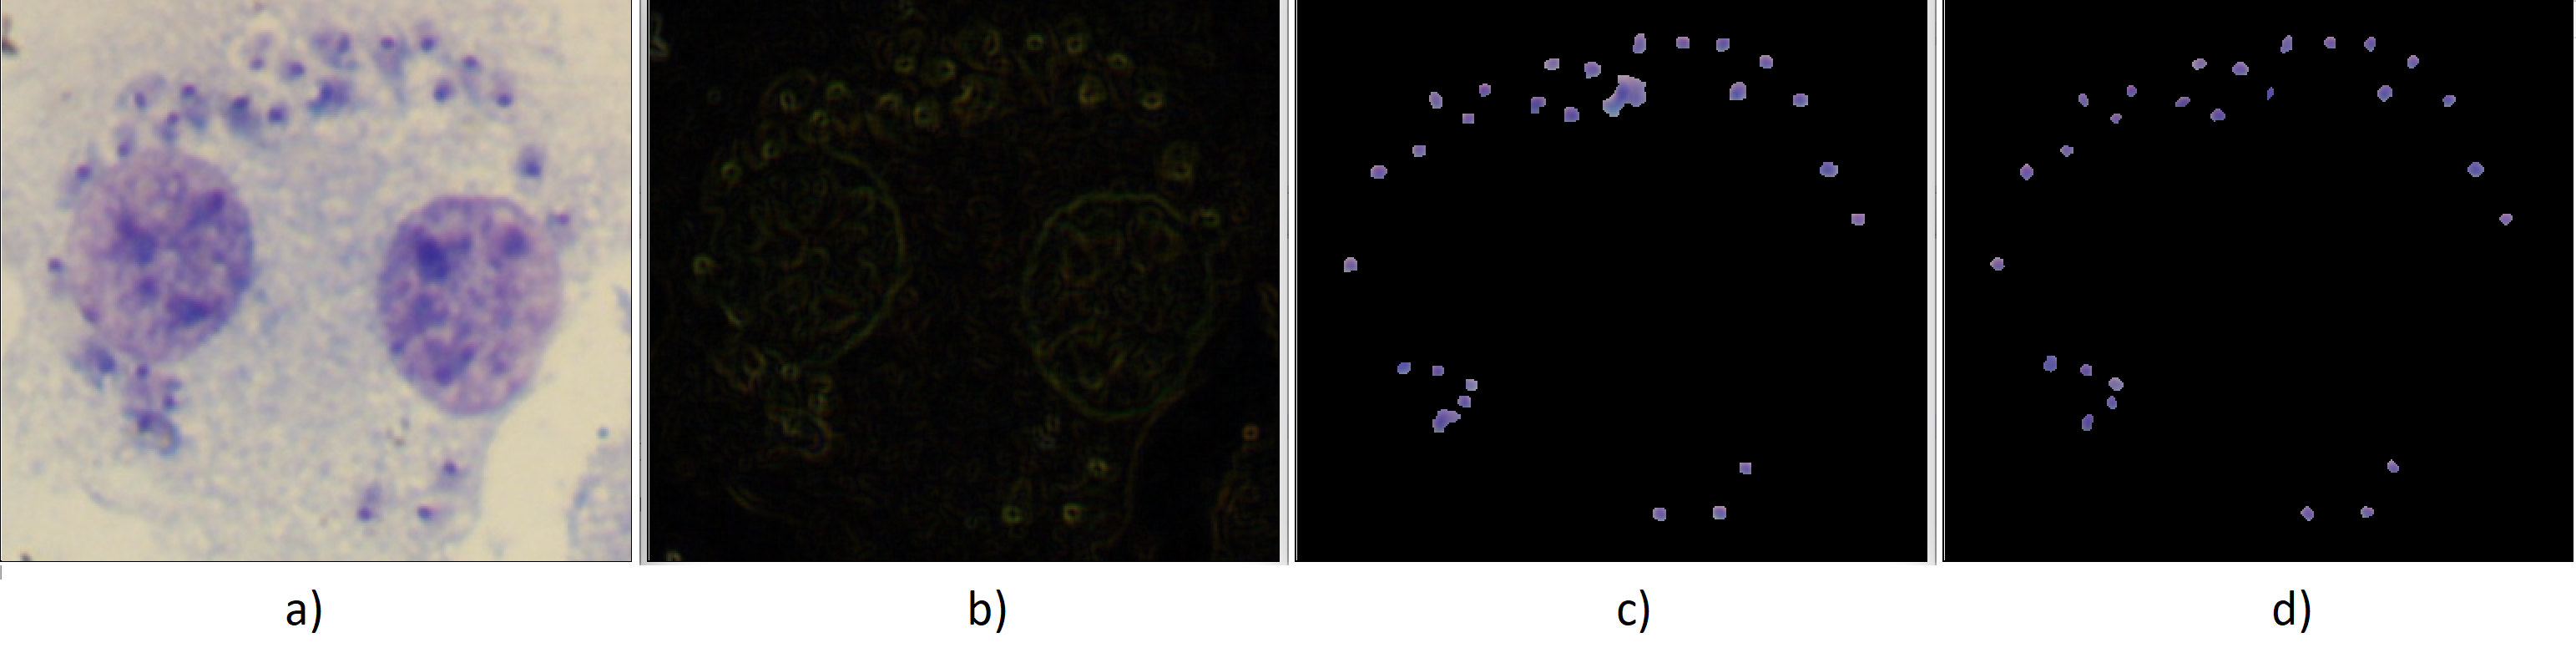
\includegraphics[width=150mm]{./imagenes/ejemplo-medialab.png}
\caption{Resultados obtenidos en el espacio de Color CIELab}
\label{exp:lab}
\end{figure}

\subsubsection{Comparación con imágenes en escala de grises}

Los resultados de la implementación utilizando el algoritmo de Vincent y Soille en escala de grises en la Figura \ref{exp:gris} muestran como los amastigotes segmentados en la esquina inferior izquierda en \ref{exp:gris}(c) poseen un tamaño mayor a lo que se ve en la segmentación ideal y en comparación con la segmentación realizada en el espacio CIELab.
\begin{figure}[h]
\centering
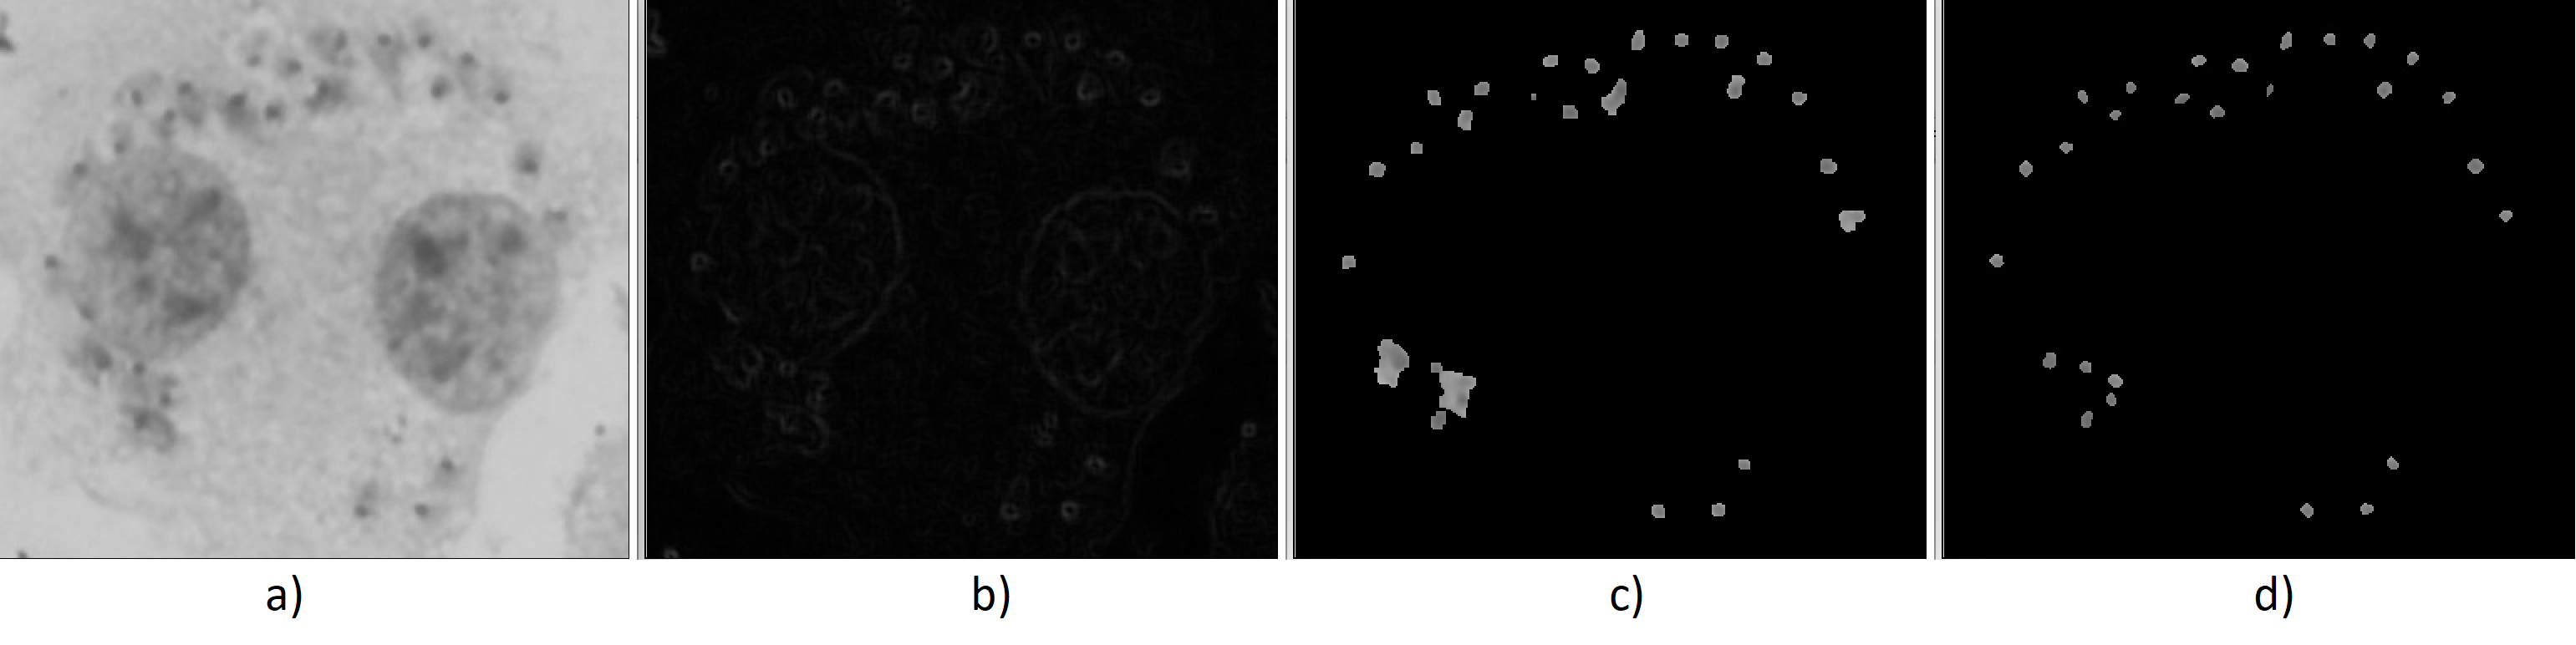
\includegraphics[width=150mm]{./imagenes/ejemplo-gris.png}
\caption{Resultados obtenidos utilizando el algoritmo de Vincent y Soille}
\label{exp:gris}
\end{figure}

En base a un análisis visual de los resultados se nota que los amastigotes segmentados tienden a ser de mayor tamaño que los esperados en la imagen ideal, esta tendencia se mantiene tanto en escala de gris como en CIELab pero en este último espacio se ve un tamaño más cercano a la imagen ideal, esto refleja la tendencia obtenida en las tablas anteriores.

\subsubsection{Comparación con imágenes a color}

Los resultados de la implementación utilizando el algoritmo de Meyer en el espacio de color RGB se pueden observar en la Figura \ref{exp:rgb}. 
\begin{figure}[h]
\centering
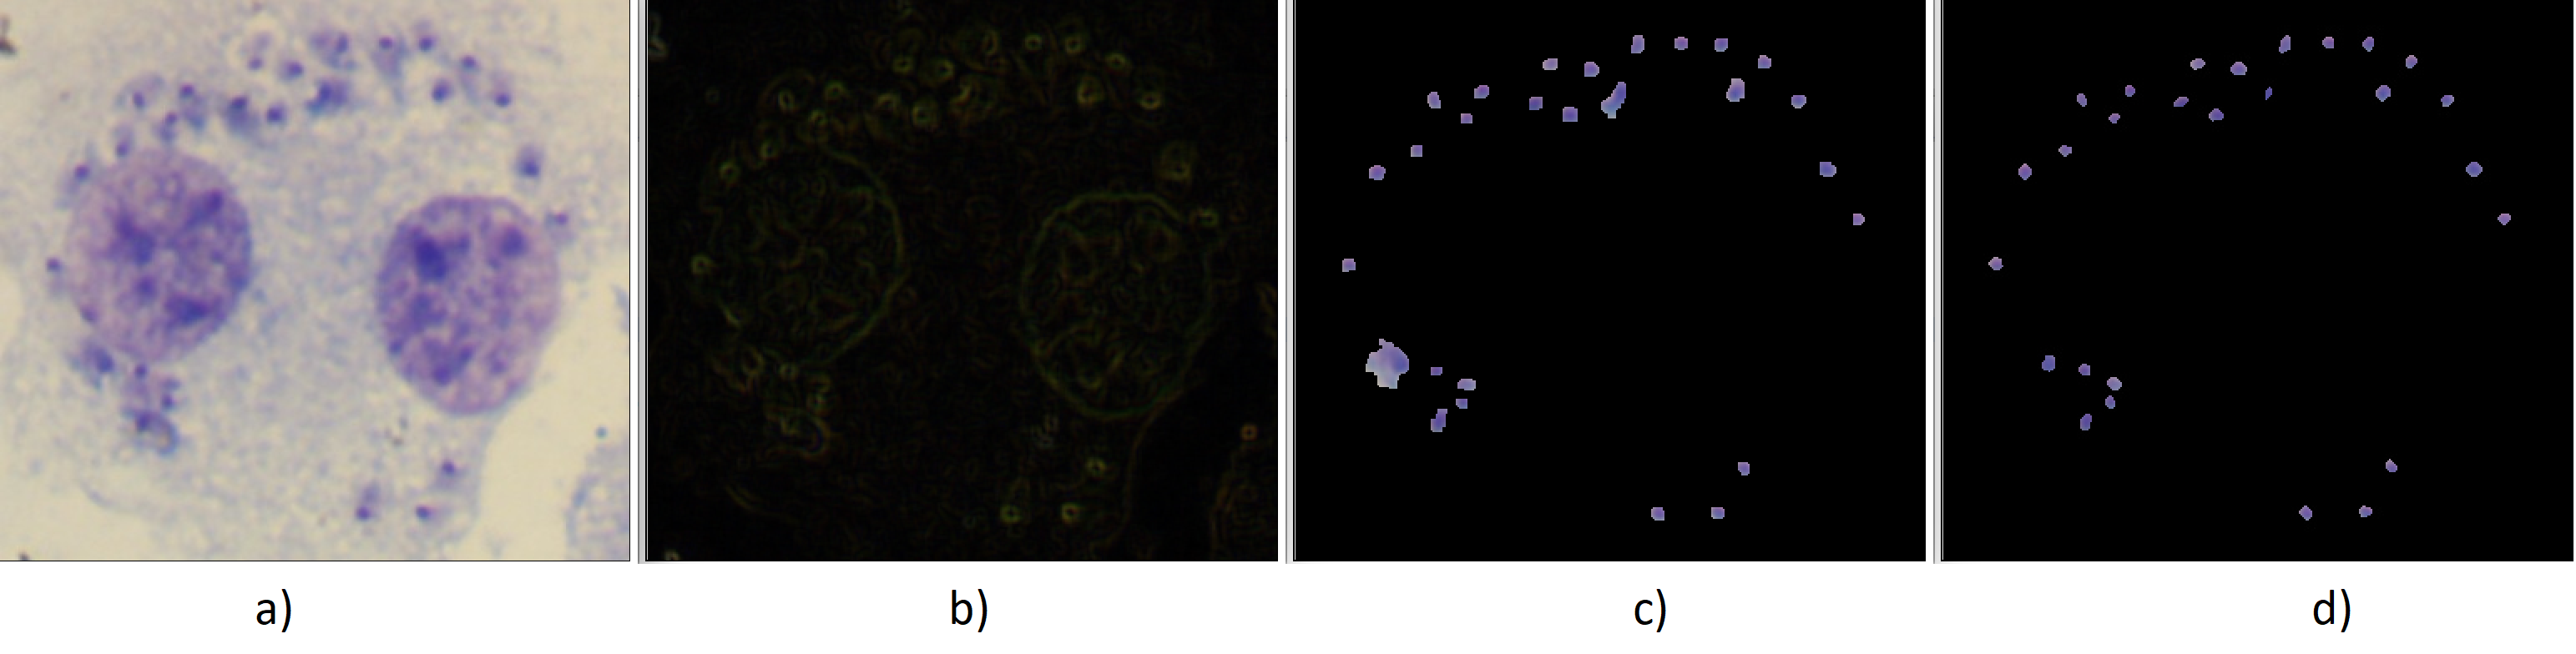
\includegraphics[width=150mm]{./imagenes/ejemplo-rgb.png}
\caption{Resultados obtenidos utilizando el algoritmo de Meyer}
\label{exp:rgb}
\end{figure}

Realizando un análisis visual de los resultados se puede ver que presenta la misma tendencia que al realizar la segmentación en escala de grises o en el espacio CIELab. Los amastigotes segmentados poseen un tamaño mayor al esperado en la imagen ideal así como lo indica la alta presencia de $FP$ en los resultados numéricos.

Comparando con los resultados obtenidos en escala de grises se puede ver una mejora al utilizar el color y comparando con la segmentación en el espacio de color CIELab se puede ver un resultado similar, tomando los amastigotes segmentados en la esquina inferior izquierda existe un mayor error de incremento de tamaño en el espacio de color RGB en comparación con el espacio de color CIELab.


En la Figura \ref{img:r1}(a) se muestra la imagen original y en \ref{img:r1}(b) la segmentación ideal.

\begin{figure}[H]
\centering
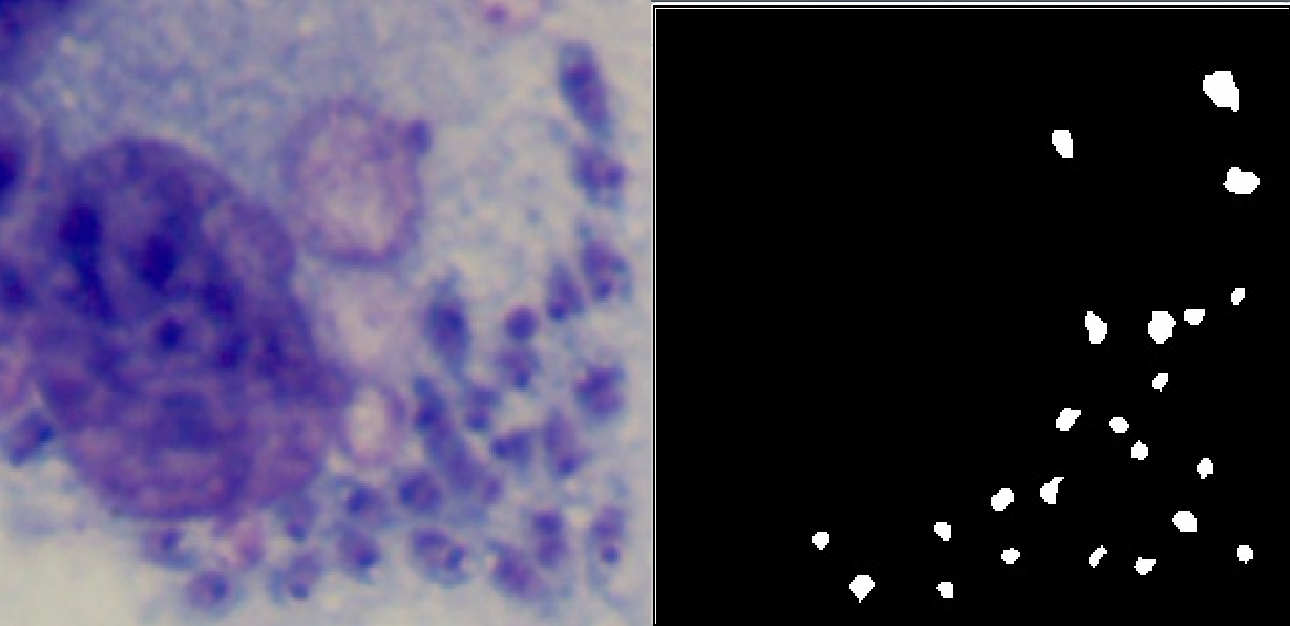
\includegraphics[width=100mm]{./imagenes/r1.png}
\caption{(a) Imagen original (b) Segmentación ideal}
\label{img:r1}
\end{figure}

En la Figura \ref{img:r2}(a) se muestra la segmentación obtenida en el espacio CIELab con el ordenamiento de la distancia a la mediana y en la Figura \ref{img:r2}(b) el espacio RGB utilizando el ordenamiento lexicógrafo, el cual obtuvo los mejores resultados entre los distintos espacios de color y ordenamientos que no utilizan el espacio CIELab. Se puede ver cómo la segmentación en el espacio de color CIELab logra delimitar los objetos con mayor precisión. Ambos métodos generan segmentaciones de los cuerpos de mayor tamaño que en la segmentación ideal, pero este error es menor en las segmentaciones con el espacio de color CIELab.

\begin{figure}[H]
\centering
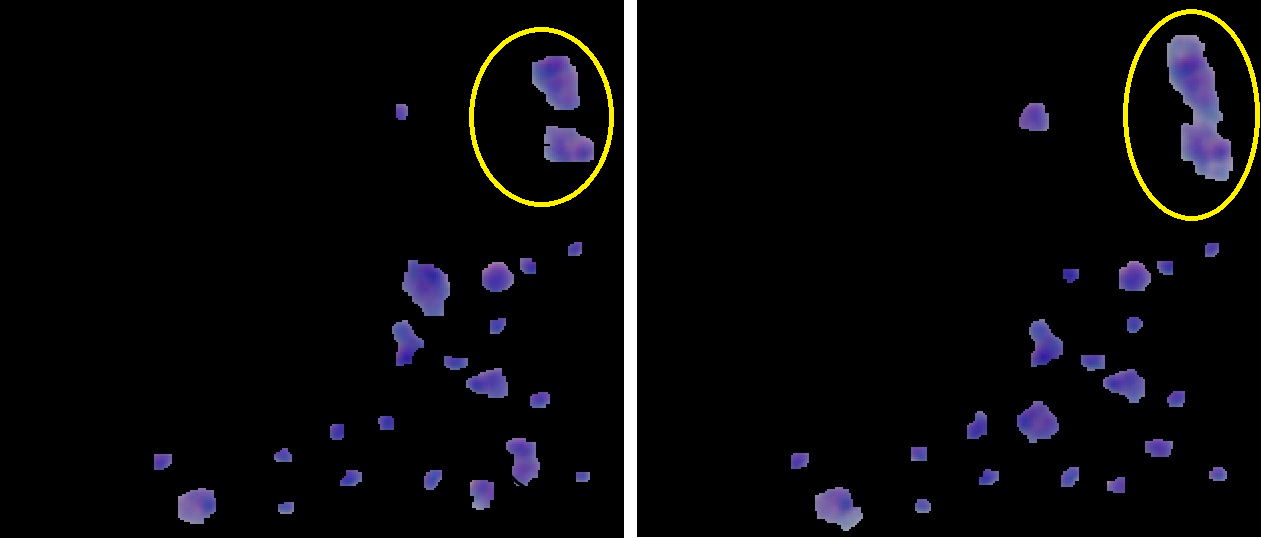
\includegraphics[width=100mm]{./imagenes/r2.png}
\caption{(a) Segmentación en CIELab (b) Segmentación en RGB}
\label{img:r2}
\end{figure}
